\documentclass[blind]{psta}
\usepackage{xargs}
\usepackage{cleveref}
\input{definitions}

% Предварительные классификаторы: перед подачей их следует подтвердить.
\subjclass[UDC]{519.245:519.217.2}
\subjclass[2020]{62L20; 60J20, 65C40}
\ArticleType{RAR}
\JournalRubric{7}

% Вся титульная информация, как в официальном шаблоне, находится в преамбуле.
% Перед подачей следует заполнить TODO-поля и согласовать состав авторов.
\Russian
\title[RR-экстраполяция в линейной стохастической аппроксимации]
{Экстраполяция Ричардсона--Ромберга для статистического вывода
в~линейной стохастической аппроксимации}

% Класс ожидает после имени ещё одно имя или отчество. Этот пустой маркер
% позволяет корректно указать автора без выдуманного отчества.
\makeatletter
\newcommand{\NoMiddleName}{\@ifnextchar.{\@gobble}{}}
\makeatother
\author{Гайнанов, {Д}аниил \NoMiddleName}
\address{\href{https://www.hse.ru}{Национальный исследовательский университет
«Высшая школа экономики»}, Москва, Россия}
% \email{TODO}
% \orcid{TODO}
% \info{TODO: 4--7 строк о статусе, научных интересах и достижениях.}
% \image{pics/TODO-author-photo}
% \CRediT{1,2,3,4,5,6,8,9,10,11}{100\%}

\begin{abstract}
Рассматривается статистический вывод для линейной стохастической аппроксимации
с постоянным шагом и марковским шумом. Усреднение Поляка--Рупперта снижает
дисперсию, но не устраняет смещение порядка шага. Поэтому при естественном
для постоянного шага выборе $\alpha\asymp n^{-1/2}$ нормированное смещение
$\sqrt n\,\alpha$ не исчезает и центрированная нормальная аппроксимация может
быть неточной. Мы запускаем рекурсии с шагами $\alpha$ и $2\alpha$ на одной
траектории и объединяем их средние экстраполяцией
Ричардсона--Ромберга. Она сокращает ведущий член смещения, сохраняя
асимптотическую дисперсию. Основной результат статьи --- неасимптотическая
гауссовская аппроксимация скалярных проекций RR-среднего после отбрасывания
первой половины траектории, как в Levin, Naumov и Samsonov. Граница явно
зависит от $n$, шага $\alpha$ и размерности $d$ и тем самым показывает
компромисс между забыванием начальной точки и остаточным смещением.
При стандартных условиях устойчивости и равномерной геометрической
эргодичности её специализация к $\alpha=c/\sqrt n$ даёт оценку расстояния
Колмогорова
$\dK\lesssim_{\log{n}}C_{\rm G}(d)n^{-1/4}$. Контроль остаточного члена в разложении
ошибки для итераций Ричардсона--Ромберга опирается на оценки моментов высокого
порядка, полученные Levin, Naumov и Samsonov; новый распределительный шаг
основан на пуассоновской мартингальной аппроксимации. В экспериментах RR
устраняет видимый сдвиг нормированной статистики и возвращает покрытие
скалярных 95\%-х интервалов к уровню 94--95\% без заметного увеличения ширины.
\end{abstract}
\keywords{линейная стохастическая аппроксимация,
марковский шум, экстраполяция Ричардсона--Ромберга,
гауссовская аппроксимация, оценка Берри--Эссеена,
доверительные интервалы, долгосрочная ковариация}

\English
\title[RR extrapolation in linear stochastic approximation]
{Richardson--Romberg Extrapolation for Statistical Inference
in Linear Stochastic Approximation}

\author{Gainanov, Danil \NoMiddleName}
\address{\href{https://www.hse.ru/en/}{HSE University}, Moscow, Russia}
% \email{TODO}
% \orcid{TODO}
% \info{TODO: 4--7 lines on status, research interests, and achievements.}
\headlineauthors{Д.~Гайнанов}{Danil Gainanov}

\begin{abstract}
We study statistical inference for constant-stepsize linear stochastic
approximation driven by Markovian observations. Polyak--Ruppert averaging
reduces random fluctuations but does not remove the bias of order $\alpha$.
Thus, under the natural constant-stepsize choice $\alpha\asymp n^{-1/2}$,
the normalized bias $\sqrt n\,\alpha$ does not vanish and a centered Gaussian
approximation can be inaccurate. We run recursions with stepsizes $\alpha$
and $2\alpha$ on the same trajectory and combine their averages by
Richardson--Romberg extrapolation. This cancels the leading bias while
preserving the asymptotic variance. Our main result is a non-asymptotic
Gaussian approximation for scalar projections of the RR average after
discarding the first half of the trajectory, as in Levin, Naumov, and Samsonov.
The bound explicitly tracks the sample size $n$, the stepsize $\alpha$, and
the dimension $d$, thereby displaying the trade-off between forgetting
the initial condition and controlling the residual bias. Under standard
stability and uniform geometric-ergodicity conditions, its specialization to
$\alpha=c/\sqrt n$ yields the Kolmogorov-distance estimate
$\dK\lesssim_{\log{n}}C_{\rm G}(d)n^{-1/4}$. Control of the RR remainder builds on the
high-order moment bounds of Levin, Naumov, and Samsonov; the new distributional
step is based on a Poisson-equation martingale approximation.
In finite-state experiments, extrapolation removes the visible shift of the
normalized statistic and brings scalar 95\% confidence-interval coverage to
94--95\% without a material increase in width.
\end{abstract}
\keywords{linear stochastic approximation, Markovian noise,
Richardson--Romberg extrapolation, Gaussian approximation,
Berry--Esseen bound, confidence intervals, long-run covariance}

\Russian

\makeatletter
\newcommand{\AfterPeer}[1]{\if y\psta@blind\else#1\fi}
% Blind-режим класса скрывает титульные данные, но подставляет их заменители
% в бегущие колонтитулы. Оставляем штатное расположение номеров страниц,
% передавая классу пустые текстовые метки.
\if y\psta@blind
  \renewcommand{\pstamarkboth}[2]{\markboth{}{}}
\fi
\makeatother

\newtheorem{theorem}{Теорема}
\newtheorem{lemma}{Лемма}
\renewcommand{\proofname}{Доказательство}

\begin{document}
\Russian
\maketitle

\section*{Введение}

Задача линейной стохастической апроксимации (LSA) рассматриваем систему линейных уравнений $\bA \thetalim = \barb$ с неизвестным вектором $\thetalim \in \rset^d$. При этом матрица $\bA$ и вектор $\barb$ неизвестны, но имеются их зашумленные наблюдения $\{\zfuncA{Z_k}, \zfuncb{Z_k}\}_{k\in \nset}$, где $\{Z_k\}_{k \in \nset}$ - это последовательность случайных величин в пространстве $(\Zset, \Zsigma)$. В данной работе, мы предполагаем, что последовательность $\{Z_k\}_{k\in \nset}$ является Марковской цепью со стационарным распределением $\pi$, и
\begin{align*}
    \PE_\pi[\zfuncA{Z}] = \bA \eqsp, \quad \PE_\pi[\zfuncb{Z}] = \barb \eqsp.
\end{align*}
Эта задача возникает в контексте обучения с подкреплением, например, для анализа алгоритма TD-обучения (Temporal-Difference Learning) \cite{sutton:book:2018}.

Для поиска решения $\thetalim$ известен классический алгоритм Роббинса--Монро c убывающим шагом $\{\alpha_k\}$
\cite{RobbinsMonro1951}. Следуя этому методу, мы рассматриваем последовательность шагов $\{\alpha_k\}_{k \in \nset}$, период разогрева $n_0 \in \nset$, и инициализацию $\thetainit \in \rset^{d}$, затем мы определяем последовательность $\{\theta_{k} \}_{k \in \nset}$ и $\{ \btheta_{n} \}_{n \geq n_0+1}$, как
\begin{equation}
\label{eq:lsa-decreasing}
\begin{split}
\textstyle \theta_{k} &= \theta_{k-1} - \alpha_k \{ \funcA{Z_k} \theta_{k-1} - \funcb{Z_k} \} \eqsp,~~ k \geq 1, \\
\textstyle \btheta_{n} &= (n-n_0)^{-1} \sum_{k=n_0}^{n-1} \theta_{k} \eqsp, ~~n \geq n_0+1 \eqsp.
\end{split}
\end{equation}
Здесь, $\btheta_{n}$ соответствует усреднению Поляка--Рупперта \cite{ruppert1988efficient,PolyakJuditsky1992}, популярный метод для ускорения сходимости алгоритмов стохастической аппроксимации. При этом на практике постоянный шаг $\alpha_k \equiv \alpha$ удобнее, так как его проще настраивать и ошибка алгоритма с экспоненциальной скоростью забывает начальное состояние \cite{Dieuleveut2020}. За это приходится платить смещением порядка шага, что не решается даже использованием усреднения Поляка--Рупперта \cite{Polyak1990,PolyakJuditsky1992}.

Для статистического вывода важна не только величина ошибки
$\btheta_n-\thetalim$, но и её распределение. При стандартных условиях на шум
и убывающий шаг PR-среднее удовлетворяет центральной предельной теореме
\cite{PolyakJuditsky1992,Samsonov2025}: для любого фиксированного направления
$u\in\rset^d$
\begin{equation}\label{eq:intro-clt}
 T_n(u):=\frac{\sqrt n\,u^\transpose(\btheta_n-\thetalim)}{\sigma(u)}
 \xrightarrow{\,d\,}\gauss(0,1),
\end{equation}
где $\sigma^2(u)$ --- асимптотическая дисперсия проекции.
Этот предел лежит в основе построения доверительных интервалов. Для конечного
$n$ их точность определяется близостью закона $T_n(u)$ к стандартному
нормальному закону. Например, в расстоянии Колмогорова эта близость измеряется
величиной
\[
 \dK\bigl(T_n(u),\gauss(0,1)\bigr)
 =\sup_{x\in\rset}\absD{\PP\{T_n(u)\leq x\}-\Phi(x)}.
\]
Неасимптотическая нормальная аппроксимация даёт явную, стремящуюся к нулю
границу на это расстояние. При постоянном шаге именно стационарное смещение
затрудняет такую аппроксимацию, центрированную в $\thetalim$.

Для PR-усреднённого TD-обучения с убывающим шагом в \cite{Srikant2024} получена
неасимптотическая оценка в расстоянии Вассерштейна; оптимизация приведённой
там границы по скорости убывания шага даёт порядок
$\sqrt{\log n}\,n^{-1/6}$. Для общей LSA с убывающим шагом и марковским шумом
в \cite{Samsonov2025} установлена оценка Берри--Эссеена для
скалярных проекций PR-среднего: при $\alpha_k\asymp k^{-3/4}$ получено
$\dK\lesssim_{\log{n}}n^{-1/4}$. По степени
$n$ эта граница быстрее, но результаты сформулированы в разных метриках.
Однако, насколько нам известно, для усреднения Поляка--Рупперта с постоянным
шагом оценка в расстоянии Колмогорова ранее получена не была.

% В \cite{Wang2026SteadyState} постоянный шаг и марковский шум рассматриваются
% для другого объекта --- стационарного закона масштабированной последней
% итерации; полученная для него оценка в расстоянии Вассерштейна имеет порядок
% $\sqrt{\alpha}\log(1/\alpha)$. Она не охватывает PR-среднее на конечной
% выборке из произвольной начальной точки. Поэтому, насколько нам
% известно, для такого PR-среднего с постоянным шагом оценка в расстоянии
% Колмогорова, центрированная в $\thetalim$, ранее получена не была.

Для постоянного шага препятствием служит стационарное смещение, которое не
устраняется PR-усреднением \cite{Dieuleveut2020,Huo2024,Levin2026} и может
замедлять сходимость в центральной предельной теореме. При этом, экстраполяция Ричардсона--Ромберга (RR) помогает уменьшить это смещение. Для
этого PR-усреднения двух рекурсий \eqref{eq:lsa-decreasing} с постоянными шагами
$\alpha$ и $2\alpha$, построенных на одной траектории, объединяются в
комбинацию $2\btheta^{(\alpha)}-\btheta^{(2\alpha)}$. В
\cite{Levin2026} для такой RR-оценки получены оценки моментов высокого порядка,
показывающие, что сокращение ведущего смещения улучшает зависящий от
$\alpha$ остаточный член. Это позволяет получить быструю
сходимость в центральной предельной теореме при постоянном шаге; ниже мы
получаем соответствующий неасимптотический результат.

Цель настоящей работы --- преобразовать эти моментные оценки в
неасимптотическую нормальную аппроксимацию. Используя пуассоновскую
мартингальную аппроксимацию и сглаживающее неравенство из
\cite{Samsonov2025}, мы получаем оценку скорости в ЦПТ с отслеживанием
зависимости от $n$, шага $\alpha$ и размерности $d$. Выбор шага и следующий
из основной оценки порядок обсуждаются после формулировки Теоремы.

Эксперименты иллюстрируют основной механизм: RR исправляет центр почти без
изменения ширины доверительного интервала.

\section{Линейная стохастическая аппроксимация с марковским шумом и экстраполяция Ричардсона-Ромберга}\label{sec:model}

Пусть $(Z_k)_{k\geq 0}$ --- однородная марковская цепь с переходным ядром
$\MKQ$ на полном сепарабельном метрическом пространстве $\Zset$ с борелевской
сигма-алгеброй $\Zsigma$ и инвариантным распределением $\pi$. Линейная
стохастическая аппроксимация с постоянным шагом $\alpha>0$ имеет вид
\begin{equation}\label{eq:lsa}
 \theta_k^{(\alpha)}=\theta_{k-1}^{(\alpha)}
 -\alpha\bigl(\zfuncA{Z_k}\theta_{k-1}^{(\alpha)}-\zfuncb{Z_k}\bigr).
\end{equation}
Обозначим $\PE_\pi[\zfuncA{Z}]=\bA$ и
$\PE_\pi[\zfuncb{Z}]=\barb$. Искомый параметр $\thetalim$ задаётся
уравнением $\bA\thetalim=\barb$. Постоянный шаг
обеспечивает геометрическое затухание начальной ошибки, но порождает
стационарное смещение относительно $\thetalim$.

Нам понадобятся три стандартных условия, совпадающие с базовыми условиями
\cite{Levin2026}: на перемешивание цепи, устойчивость системы и шум в оптимальной точке.

\begin{enumerate}
\item Цепь равномерно геометрически эргодична. В частности, её коэффициент
Добрушина удовлетворяет
\[
 \dobru{\MKQ^k}
 :=\sup_{z,z'}\frac12\tvnorm{
 \MKQ^k(z,\cdot)-\MKQ^k(z',\cdot)}
 \leq(1/4)^{\floor{k/\taumix}},\qquad k\geq1.
\]
$\taumix$ --- число шагов, за которое коэффициент Добрушина уменьшается не
менее чем до $1/4$; условие также влечёт единственность $\pi$.
\item Матрица $-\bA$ гурвицева, а функции $\funcAw$ и $\funcbw$ ограничены.
Существует матрица $Q=Q^\transpose\succ0$ и числа $a>0$,
$\alpha_\infty>0$ такие, что, после возможного уменьшения
$\alpha_\infty$,
\begin{equation}\label{eq:contraction}
 \norm{I-\alpha\bA}[Q]^2\leq 1-\alpha a,
 \qquad \alpha a\leq\tfrac12,
 \qquad 0\leq\alpha\leq\alpha_\infty .
\end{equation}
Гурвицевость обеспечивает единственность $\thetalim$, а
\eqref{eq:contraction} даёт
$\norm{(I-\alpha\bA)^k}[Q]\brel\leq(1-\alpha a)^{k/2}$ и тем самым контролирует
вклад инициализации.
\item Центрированный шум в оптимальной точке
$\funcnoise{z}=\zmfuncA{z}\thetalim-\zmfuncb{z}$ ограничен, где мы полагаем
\begin{align*}
  \zmfuncA{z} = \zfuncA{z} - \bA\eqsp, \quad \zmfuncb{z} = \zfuncb{z} - \barb \eqsp,
\end{align*}
и по построению $\PE_\pi[\funcnoise{Z}]=0$.
\end{enumerate}

Здесь $\norm{x}[Q]^2=x^\transpose Qx$, матричная $Q$-норма индуцирована этой
векторной нормой, а без индекса используется евклидова или спектральная
норма. Все параметры задачи в дальнейшем считаются фиксированными. Условия 1
и 3, в частности, гарантируют абсолютную сходимость ряда, определяющего ковариационную матрицу
\begin{equation}\label{eq:sigmam}
 \noisecovmarkov=\PE_\pi[\funcnoise{Z_0}\funcnoise{Z_0}^\transpose]
 +2\sum_{\ell \geq 1}\PE_\pi\!\left[
 \funcnoise{Z_0}\funcnoise{Z_\ell}^\transpose
 \right].
\end{equation}
Будем считать матрицу $\noisecovmarkov$ положительно определённой и обозначим
\begin{equation}\label{eq:Cepsilon}
 \Const{\varepsilon}:=\lambda_{\min}(\noisecovmarkov)^{-1/2}.
\end{equation}
Асимптотическая ковариационная матрица усреднённой оценки имеет вид
\begin{equation}\label{eq:sigmainfty}
 \Sigma_\infty=\bA^{-1}\noisecovmarkov\bA^{-\transpose}.
\end{equation}
Это предельная ковариационная матрица PR-усреднения. Для направления
$u\in\sphere^{d-1}$ положим
\begin{equation}\label{eq:directional-variance}
 \sigma^2(u):=u^\transpose\Sigma_\infty u.
\end{equation}
Пусть $0\leq n_0<n$. После разогрева усредняются последние $n-n_0$
итераций:
\begin{equation}\label{eq:pr}
 \btheta_{n,n_0}^{(\alpha)}
 =\frac1{n-n_0}\sum_{k=n_0}^{n-1}\theta_k^{(\alpha)}.
\end{equation}
Параметр разогрева $n_0$ позволяет с экспоненциальной по $n_0$ скоростью забывать начальное состояние. 
Усреднение Поляка-Рупперта позволяет получать оптимальную асимптотическую дисперсию в задачах стохастической аппроксимации \cite{PolyakJuditsky1992}. Две рекурсии \eqref{eq:lsa} запускаются из одной детерминированной точки $\thetainit$,
используют одну траекторию $(Z_k)$ и объединяются в следующую оценку
\begin{equation}\label{eq:rr}
 \btheta_{n,n_0}^{(\alpha, \RR)}
 =2\btheta_{n,n_0}^{(\alpha)}-
 \btheta_{n,n_0}^{(2\alpha)}.
\end{equation}

Для достаточно малого $\alpha$ совместная цепь
$(\theta_k^{(\alpha)},Z_{k+1})$ имеет единственное стационарное распределение
\cite[Теорема~1]{Levin2026}. Если $\theta_\infty^{(\alpha)}$ обозначает его
$\theta$-координату, то
\begin{equation}\label{eq:stationary-bias}
 \PE[\theta_\infty^{(\alpha)}]
 =\thetalim+\alpha\Delta+O(\alpha^{3/2}) \eqsp,
\end{equation}
где $\Delta$ --- вектор, не зависящий от $\alpha$. Следовательно,
\[
 2\PE[\theta_\infty^{(\alpha)}]-
 \PE[\theta_\infty^{(2\alpha)}]
 =\thetalim+O(\alpha^{3/2}).
\]
Таким образом, RR сокращает смещение порядка $\alpha$. При
$\alpha\asymp n^{-1/2}$ нормированное смещение обычного среднего имеет
порядок $\sqrt n\,\alpha\asymp1$, а после RR --- порядок
$\sqrt n\,\alpha^{3/2}\asymp n^{-1/4}$.

В следующем разделе будет использоваться та же схема разогрева, что и в
\cite[Теорема~2]{Levin2026}. Считаем $n$ чётным и полагаем
\begin{equation}\label{eq:half-burn-in}
 n_0=n/2.
\end{equation}
Таким образом, первые $n/2$ итераций отбрасываются, а последние $n/2$
усредняются. Для ошибки
\[
 \bA(\btheta_{n,n_0}^{(\alpha, \RR)}-\thetalim)
\]
непосредственно применима оценка \cite[Теорема~2]{Levin2026}.
В следующем разделе эта оценка вместе с мартингальной аппроксимацией
марковского шума используется для получения неасимптотической ЦПТ для итераций Ричардсона-Ромберга.


\section{Гауссовская аппроксимация RR+PR}\label{sec:theory}

Для достаточно малого $w$ совместная цепь
$(\theta_k^{(w)},Z_{k+1})$ имеет единственный инвариантный закон
\cite[Theorem~1]{Levin2026}. Обозначим через $\theta_\infty^{(w)}$
его $\theta$-координату. Из разложения
\[
\E\theta_\infty^{(w)}
=\theta^\star+w\Delta+O(w^{3/2})
\]
следует, что комбинация \eqref{eq:rr} сокращает член $w\Delta$
\cite[Corollary~1]{Levin2026}. Для распределительного результата одного
сокращения ожиданий недостаточно: требуется отделить ведущую марковскую сумму
от нелинейного остатка и сравнить её дисперсию с \eqref{eq:sigmainfty}.

\subsection{Веса и детерминированная ковариационная прокси}

Положим $B_w=I-w\Abar$. Вклад шума, возникшего в момент $l$, в среднее по
окну $k=n_0,\ldots,n-1$ имеет детерминированный вес
\begin{equation}\label{eq:burned-weight}
Q_{l;n_0,n}^{(w)}
=\begin{cases}
\Abar^{-1}(B_w^{\,n_0-l}-B_w^{\,n-l}),&1\leq l<n_0,\\[2mm]
\Abar^{-1}(I-B_w^{\,n-l}),&n_0\leq l\leq n-1.
\end{cases}
\end{equation}
RR-вес равен
\[
Q_l^{\RR}=2Q_{l;n_0,n}^{(\alpha)}
-Q_{l;n_0,n}^{(2\alpha)}.
\]
Из \eqref{eq:contraction} и геометрических сумм следуют фиксированные
константы\linebreak $C_Q,C_V<\infty$, не зависящие от $n$, $n_0$ и $\alpha$, для которых
\begin{equation}\label{eq:weight-controls}
\max_{1\leq l<n}\norm{Q_l^{\RR}}\leq C_Q,\qquad
\sum_{l=1}^{n-2}\norm{Q_{l+1}^{\RR}-Q_l^{\RR}}
\leq C_V/a^2.
\end{equation}
Поэтому ведущая, линейная по $\eps$ часть нормированной ошибки имеет вид
\begin{equation}\label{eq:leading-weighted-sum}
W_{n,n_0}^{\RR}
=-\frac1{\sqrt m}\sum_{l=1}^{n-1}Q_l^{\RR}\eps(Z_l).
\end{equation}
Сумма содержит и индексы до $n_0$: соответствующие веса экспоненциально
затухают, но не равны нулю. Множитель $1/m$ в следующей ковариационной прокси
появляется из нормировки $1/\sqrt m$ в
\eqref{eq:leading-weighted-sum}, то есть из длины окна PR-усреднения, а не из
числа индексов в шумовой сумме.

\begin{lemma}[Сравнение ковариационной прокси]
\label{lem:variance}
Пусть выполнено \eqref{eq:contraction}, $0<\alpha$,
$2\alpha\leq\alpha_\infty$ и $\norm{\SigmaM}<\infty$. Определим
\begin{equation}\label{eq:sigma-proxy}
\Sigma_{n,n_0}^{\mathrm{bRR}}
=\frac1m\sum_{l=2}^{n-1}
Q_l^{\RR}\SigmaM(Q_l^{\RR})^\top,\qquad
\sigma_{n,n_0}^2(u)
=u^\top\Sigma_{n,n_0}^{\mathrm{bRR}}u.
\end{equation}
Положим $\sigma_{n,n_0}(u)=\sqrt{\sigma_{n,n_0}^2(u)}$.
Тогда существует фиксированная константа $C_{\rm var}<\infty$ такая, что
\begin{equation}\label{eq:variance-bound}
\norm{\Sigma_{n,n_0}^{\mathrm{bRR}}-\Sigma_\infty}
\leq\frac{C_{\rm var}}{m\alpha a},\qquad
|\sigma_{n,n_0}^2(u)-\sigma^2(u)|
\leq\frac{C_{\rm var}\norm u^2}{m\alpha a}.
\end{equation}
Константа зависит только от $Q,\Abar$ и $\norm{\SigmaM}$.
\end{lemma}

\begin{proof}
Пусть $\rho_\alpha=(1-\alpha a)^{1/2}$. Из
\eqref{eq:burned-weight} и \eqref{eq:contraction} получаем
\[
\norm{Q_l^{\RR}-\Abar^{-1}}
\lesssim\rho_\alpha^{\,n-l}\quad(l\geq n_0),\qquad
\norm{Q_l^{\RR}}
\lesssim\rho_\alpha^{\,n_0-l}\quad(l<n_0).
\]
Геометрические суммы первых и вторых степеней этих оценок имеют порядок
$(\alpha a)^{-1}$. В части после разогрева раскрываем
\[
Q_l^{\RR}\SigmaM(Q_l^{\RR})^\top-\Sigma_\infty
\]
по степеням $Q_l^{\RR}-\Abar^{-1}$; предшествующую часть оцениваем по энергии
$\sum_{l<n_0}\norm{Q_l^{\RR}}^2$. Не более двух граничных позиций дают
$O(m^{-1})$, которое поглощается правой частью
\eqref{eq:variance-bound}. После деления на $m$ получаем первое неравенство,
а второе следует из $|u^\top Hu|\leq\norm H\norm u^2$.
\end{proof}

\subsection{Мартингал и моментная оценка остатка}

Пусть $\mathsf P$ --- переходное ядро цепи. Уравнение Пуассона имеет
ограниченное решение
\[
\widehat\eps=\sum_{j\geq0}\mathsf P^j\eps,\qquad
\widehat\eps-\mathsf P\widehat\eps=\eps,\qquad
\norm{\widehat\eps}_\infty\lesssim\tmix\norm\eps_\infty .
\]
Кроме того,
\[
\mathcal V_\eps(z)=\mathsf P(\widehat\eps\widehat\eps^\top)(z)
-(\mathsf P\widehat\eps)(z)(\mathsf P\widehat\eps)(z)^\top,
\qquad \E_\pi\mathcal V_\eps(Z)=\SigmaM.
\]
Для $2\leq l\leq n-1$ положим
\[
\Delta M_l^{\mathrm{bRR}}
=Q_l^{\RR}\{\widehat\eps(Z_l)
-\mathsf P\widehat\eps(Z_{l-1})\},\qquad
M_{n,n_0}^{\mathrm{bRR}}
=\sum_{l=2}^{n-1}\Delta M_l^{\mathrm{bRR}} .
\]
Это мартингальные разности. Суммирование Абеля даёт
\begin{equation}\label{eq:poisson-decomp}
W_{n,n_0}^{\RR}
=-\frac{M_{n,n_0}^{\mathrm{bRR}}}{\sqrt m}+D_{2,n,n_0},
\qquad
\norm{D_{2,n,n_0}}_\infty\lesssim\frac{\tmix}{\sqrt m}.
\end{equation}
Здесь
\[
D_{2,n,n_0}=-\frac1{\sqrt m}\left\{
Q_1^{\RR}\widehat\eps(Z_1)
+\sum_{l=1}^{n-2}(Q_{l+1}^{\RR}-Q_l^{\RR})
\mathsf P\widehat\eps(Z_l)\right\};
\]
его оценка следует из \eqref{eq:weight-controls}.
Здесь и далее $\lesssim$ не скрывает зависимости от
$\tmix,n,p,\alpha$; фиксированные величины
$C_A,\kappa_Q,a,\norm{\Abar^{-1}}$ и $\norm\eps_\infty$ считаются
константами задачи.

Предсказуемая квадратичная вариация этого мартингала равна
\begin{equation}\label{eq:bracket}
\langle M\rangle_{n,n_0}
:=\sum_{l=2}^{n-1}\E[\Delta M_l^{\mathrm{bRR}}
(\Delta M_l^{\mathrm{bRR}})^\top\mid\mathcal F_{l-1}]
=\sum_{l=2}^{n-1}Q_l^{\RR}\mathcal V_\eps(Z_{l-1})(Q_l^{\RR})^\top.
\end{equation}

\begin{lemma}[Концентрация случайной скобки]\label{lem:bracket}
При условиях леммы~\ref{lem:variance} и условиях 1, 3 для всех $p\geq2$,
всех $u$ и любого начального распределения цепи
\begin{equation}\label{eq:bracket-bound}
\norm{u^\top\langle M\rangle_{n,n_0}u
-m\sigma_{n,n_0}^2(u)}_{L_p}
\lesssim C_Q^2\norm u^2\norm\eps_\infty^2
\tmix^{5/2}\sqrt{pn}.
\end{equation}
Здесь и в дальнейшем $\lesssim$ не скрывает зависимости от
$\tmix,n,p,\alpha$.
\end{lemma}

\begin{proof}
Для $2\leq l<n$ положим
\[
g_l(z)=u^\top Q_l^{\RR}
\{\mathcal V_\eps(z)-\SigmaM\}(Q_l^{\RR})^\top u.
\]
Из пуассоновского представления
$\norm{\mathcal V_\eps}_\infty
\lesssim\tmix^2\norm\eps_\infty^2$, поэтому
$\norm{g_l}_\infty\lesssim
C_Q^2\norm u^2\tmix^2\norm\eps_\infty^2$ и $\E_\pi g_l=0$.
Левая часть \eqref{eq:bracket-bound} есть норма
$\sum_{l=2}^{n-1}g_l(Z_{l-1})$. Неоднородное марковское неравенство
\cite[Lemma~11]{Levin2026} даёт дополнительный множитель
$\sqrt{p\tmix n}$ и завершает доказательство.
\end{proof}

\begingroup
\emergencystretch=2em
Для точной формулировки обозначим через
$\alpha_{\mathrm{P2}},\alpha_{\mathrm{C6}},
 \alpha_{\mathrm{P8}},\alpha_{\mathrm{P9}},\alpha_{\mathrm{C4}}$
пороги из Proposition~2, Corollary~6, Propositions~8--9 и Corollary~4
расширенной версии \cite{Levin2026} при используемых ниже порядках, а через
$\alpha_{\mathrm{P5}}(r,\tmix)$ --- порог Proposition~5 для момента порядка
$r$. Положим
\endgroup
\[
\begin{aligned}
\alpha_*(p,q,\tmix)=\min\{&\alpha_{\mathrm{P2}},\alpha_{\mathrm{C6}},
 \alpha_{\mathrm{P5}}(p,\tmix),\alpha_{\mathrm{P5}}(2p,\tmix),\\[-1mm]
 &\alpha_{\mathrm{P8}},\alpha_{\mathrm{P9}},\alpha_{\mathrm{C4}}\}.
\end{aligned}
\]
\begin{equation}\label{eq:alpha-adm}
\begin{aligned}
\alpha_{\mathrm{adm}}(p,q,\tmix)
 &=\min\Biggl\{\alpha_\infty,\frac1{2\norm{\Abar}},
 \alpha_*(p,q,\tmix),\alpha_{\rm prod}(p),\\[-1mm]
 &\hspace{25mm}\alpha_{\rm prod}(2p),\frac1{2a},
 \frac1{2a\tmix}\Biggr\}.
\end{aligned}
\end{equation}
Аргументы остальных исходных порогов выбираются ровно при тех порядках
моментов, при которых они используются, и опущены только для читаемости.

Для $w\in\{\alpha,2\alpha\}$ определим компоненты разложения второго порядка.
Положим $J_0^{(\ell,w)}=0$ и $H_0^{(2,w)}=0$, а также
\begin{align*}
J_k^{(0,w)}&=B_wJ_{k-1}^{(0,w)}-w\eps(Z_k),\\
J_k^{(\ell,w)}&=B_wJ_{k-1}^{(\ell,w)}
-w\widetilde A(Z_k)J_{k-1}^{(\ell-1,w)},\quad \ell=1,2,\\
H_k^{(2,w)}&=(I-wA(Z_k))H_{k-1}^{(2,w)}
-w\widetilde A(Z_k)J_{k-1}^{(2,w)}.
\end{align*}
Тогда повторная подстановка в \eqref{eq:lsa} даёт точное равенство
\begin{equation}\label{eq:depth-two}
\begin{aligned}
\theta_k^{(w)}-\theta^\star
 &=\Gamma_{1:k}^{(w)}(\theta_0-\theta^\star)+J_k^{(0,w)}
   +R_{k,\rm fin}^{(w)},\\
R_{k,\rm fin}^{(w)}
 &=J_k^{(1,w)}+J_k^{(2,w)}+H_k^{(2,w)}.
\end{aligned}
\end{equation}

Нам понадобится один локальный переход от стационарных оценок компонент к
детерминированному старту.

\begin{lemma}[Перенос после разогрева]\label{lem:startup}
Пусть $p\geq2$, $q\geq4p$ и
$2\alpha\leq\alpha_{\mathrm{adm}}(p,q,\tmix)$. Для каждой ветви существует
стационарная двусторонняя версия $R_{k,\rm stat}^{(w)}$ и сопряжение с
конечной версией из \eqref{eq:depth-two}, равномерное по закону $Z_0$, такие,
что
\begin{equation}\label{eq:startup-pointwise}
\norm{R_{k,\rm fin}^{(w)}-R_{k,\rm stat}^{(w)}}_{L_p}
\leq A_{\rm st}(p,q,w)
\exp\!\left(-\frac{c_{\rm st}wak}{p}\right),
\end{equation}
где $c_{\rm st}>0$ фиксирована и
\begin{equation}\label{eq:Ast}
A_{\rm st}(p,q,w)=C_{\rm st}(1+d^{1/q})(p^7+p^8/a)
\tmix^5\sqrt{w/a}\,\log^3\!\frac1{wa}.
\end{equation}
Следовательно,
\begin{equation}\label{eq:startup-window}
\begin{aligned}
&\left\|\frac1{\sqrt m}\sum_{k=n_0}^{n-1}
 \begin{aligned}
 \bigl\{&2(R_{k,\rm fin}^{(\alpha)}-R_{k,\rm stat}^{(\alpha)})\\[-1mm]
 &{}-(R_{k,\rm fin}^{(2\alpha)}-R_{k,\rm stat}^{(2\alpha)})\bigr\}
 \end{aligned}\right\|_{L_p}\\
&\qquad\lesssim\frac{pA_{\rm st}(p,q,\alpha)}{\alpha a\sqrt m}
 \exp\!\left(-\frac{c_{\rm st}\alpha an_0}{p}\right).
\end{aligned}
\end{equation}
\end{lemma}

\begin{proof}
Построим стационарную координату $H^{(2,w)}$. На одной двусторонней
стационарной цепи запустим все $J$- и $H$-координаты из нуля в момент $-N$.
Corollary~4 из \cite{Levin2026} даёт инвариантный закон $J$-координат.
Сравнивая запуски из моментов $-N'$ и $-N$, $N'\geq N$, используем после
$-N$ общую траекторию цепи, то есть сопряжение с $T=0$. Покомпонентный расчёт
из доказательства Proposition~5 применим к этому синхронному сопряжению;
начальная стоимость в нём оценивается Lemmas~4, 8 и Proposition~8 при порядках
$p$ и $2p$. Условие $q\geq4p$ обеспечивает допустимость последнего порядка.
В результате, для $-N\leq r\leq0$ и $\ell=0,1,2$,
\[
\norm{\Delta J_r^{(\ell,w)}}_{L_p}
\leq A_J(p,q,w)
\exp\!\left\{-\frac{wa(r+N)}{12p}\right\},
\]
где
\[
A_J(p,q,w)\lesssim(1+d^{1/q})p^7\tmix^5
\sqrt{w/a}\,\log^3\!\frac1{wa}.
\]
Вычитая две конечнопрошлые $H$-рекурсии, получаем
\[
\Delta H_0
=\Gamma_{-N+1:0}^{(w)}H_{-N,N'}^{(2,w)}
-w\sum_{l=-N+1}^{0}\Gamma_{l+1:0}^{(w)}
\widetilde A(Z_l)\Delta J_{l-1}^{(2,w)}.
\]
Условие~4, Proposition~9 из \cite{Levin2026} и геометрическая свёртка дают
\[
\norm{\Delta H_0}_{L_p}
\lesssim\left\{B_H(p,q,w)+\frac paA_J(p,q,w)\right\}e^{-cwaN/p},
\]
где
\[
B_H(p,q,w)\lesssim(1+d^{1/q})p^{7/2}\tmix^{5/2}
 w^{3/2}\log^{3/2}\!\frac1{wa}.
\]
Следовательно, $H_{0,N}^{(2,w)}$ фундаментальна в $L_p$.
Сдвиг конструкции определяет двустороннюю стационарную координату, а оценка
$B_H$ переходит к пределу по лемме Фату. Обе RR-ветви строятся на одной
двусторонней цепи.

Теперь зададим одно сопряжение конечной и стационарной версий, пригодное для
всех оставшихся оценок. Положим $b=\lceil\tmix\rceil$. В моменты, кратные
$b$, максимально сопрягаем конечные точки двух $\mathsf P^b$-блоков;
условные распределения путей внутри блока существуют, поскольку пространство
польское. После первого совпадения используем общие переходы. Получаем липкое
блочно-коадаптированное сопряжение; момент встречи $T$ является stopping time
блочной фильтрации и
\[
\Pr(T>r)\leq C\exp(-cr/\tmix).
\]
Доказательство Proposition~5 использует для $J$-координат только это свойство,
совпадение траекторий после $T$ и равномерные моменты. Повторяя в треугольных
рекурсиях его покомпонентную подстановку и оценку события $\{T>k\}$ по
Гёльдеру, при порядках $p$ и $2p$ получаем для того же сопряжения
\begin{equation}\label{eq:J-same-coupling}
\sum_{\ell=0}^2
\norm{\Delta J_k^{(\ell,w)}}_{L_{2p}}
\leq A_J(2p,q,w)\exp(-cwak/p).
\end{equation}
Таким образом, здесь не переносится абстрактная Wasserstein-оценка на другое
сопряжение: её покомпонентный расчёт повторён для выбранного блочного
сопряжения.

\begingroup
\emergencystretch=2em
После $T$ общая будущая цепь условно по $\mathcal G_T$ имеет исходное ядро.
Поэтому условие~4 распространяется с детерминированных на
$\mathcal G_s$-измеримые векторы поточечным условливанием. В
\eqref{eq:alpha-adm} обеспечено $wa\tmix\leq1/2$. Если
$\sup_s\norm{V_s}_{L_{2p}}\leq B$, то
\par
\endgroup
\[
\norm{V_s\mathbf1_{\{T=s\}}}_{L_p}
\leq B\Pr(T=s)^{1/(2p)}
\leq CB e^{-cs/(p\tmix)}
\leq CB e^{-c'was/p}.
\]
Следовательно,
\begin{align*}
\norm{\Gamma_{T+1:k}^{(w)}V_T\mathbf1_{\{T\leq k\}}}_{L_p}
&\leq C\sum_{s=0}^k e^{-cwa(k-s)/p}
 \norm{V_s\mathbf1_{\{T=s\}}}_{L_p}\\[-1mm]
&\leq C\frac p{wa}B\,e^{-c'wak/p}.
\end{align*}
А для адаптированных $U_l$, удовлетворяющих
$\norm{U_l}_{L_{2p}}\leq B e^{-c_0wal/p}$, та же условная оценка даёт
\[
w\sum_{l=1}^k
\norm{\Gamma_{l+1:k}^{(w)}U_l\mathbf1_{\{T<l\}}}_{L_p}
\leq C\frac paB e^{-c'wak/p}.
\]

На событии $\{T\leq k\}$ имеем
\[
\Delta H_k^{(2,w)}
=\Gamma_{T+1:k}^{(w)}\Delta H_T^{(2,w)}
-w\sum_{l=T+1}^k\Gamma_{l+1:k}^{(w)}
 \widetilde A(Z_l)\Delta J_{l-1}^{(2,w)}.
\]
Первый член контролируется случайным рестартом с $B=B_H(2p,q,w)$. Во втором
берём
$U_l=\mathbf1_{\{T<l\}}\widetilde A(Z_l)\Delta J_{l-1}^{(2,w)}$ и применяем
\eqref{eq:J-same-coupling} и устойчивую свёртку. На дополнении по Гёльдеру
\[
\norm{\Delta H_k^{(2,w)}\mathbf1_{\{T>k\}}}_{L_p}
\leq C B_H(2p,q,w)e^{-ck/(p\tmix)}
\leq C B_H(2p,q,w)e^{-cwak/p}.
\]
Собирая три координаты и используя определения $A_J,B_H$, получаем
\eqref{eq:startup-pointwise} с \eqref{eq:Ast}. Суммирование по окну и
$1-e^{-c\alpha a/p}\gtrsim\alpha a/p$ дают
\eqref{eq:startup-window}.
\end{proof}

Из \eqref{eq:depth-two}, перестановки сумм в $J^{(0,w)}$ и
\eqref{eq:poisson-decomp} получаем точное разложение
\begin{equation}\label{eq:full-decomp}
\sqrt m\,u^\top
(\bar\theta_{n,n_0}^{\RR,\alpha}-\theta^\star)
=-\frac{u^\top M_{n,n_0}^{\mathrm{bRR}}}{\sqrt m}
+\mathcal R_{n,n_0}^{\RR}(u),
\end{equation}
где
\begin{align}\label{eq:composite-remainder}
\mathcal R_{n,n_0}^{\RR}(u)
&=\frac1{\sqrt m}\sum_{k=n_0}^{n-1}u^\top
\{2\Gamma_{1:k}^{(\alpha)}-\Gamma_{1:k}^{(2\alpha)}\}
(\theta_0-\theta^\star)+u^\top D_{2,n,n_0}\notag\\
&\quad+\frac1{\sqrt m}\sum_{k=n_0}^{n-1}u^\top
\{2R_{k,\rm fin}^{(\alpha)}-R_{k,\rm fin}^{(2\alpha)}\}.
\end{align}


\begin{lemma}[Момент остатка]\label{lem:remainder}
Пусть $p\geq2$ и $q\geq4p$. Предположим, что
$2\alpha\leq\alpha_{\mathrm{adm}}(p,q,\tmix)$. Обозначим
\[
L_\alpha=\log\frac1{\alpha a}.
\]
Тогда
\begin{equation}\label{eq:remainder-bound}
\norm{\mathcal R_{n,n_0}^{\RR}(u)}_{L_p}
\lesssim\norm u\,\mathcal B_R(m,n_0,p,q,\alpha),
\end{equation}
где
\begin{align}
\mathcal B_R
&=
\frac{\norm{\theta_0-\theta^\star}}{\alpha a\sqrt m}
\left\{(1-\alpha a)^{n_0/2}
+p\exp\!\left(-\frac{c_0\alpha a n_0}{p}\right)\right\}
+\frac{\tmix}{\sqrt m} \notag\\
&\quad+\tmix^2\sqrt m\,\alpha^2
+(1+d^{1/q})p^{7/2}\tmix^{5/2}
\sqrt m\,\alpha^{3/2}L_\alpha^{3/2}
+\tmix p^{3/2}\sqrt\alpha \notag\\
&\quad+\frac{\tmix^{3/2}p^3L_\alpha^{1/2}}{\sqrt{\alpha m}}
+\frac{p^2\tmix^{3/2}aL_\alpha^{1/2}}{\sqrt m}
+\frac{pA_{\mathrm{st}}(p,q,\alpha)}
{\alpha a\sqrt m}
\exp\!\left(-\frac{c_{\rm st}\alpha a n_0}{p}\right).
\label{eq:BR}
\end{align}
Постоянные $c_0,c_{\rm st}>0$ не зависят от
$\tmix,n,p,\alpha$.
\end{lemma}

\begin{proof}
В \eqref{eq:composite-remainder} начальный продукт раскладываем как
$\Gamma_{1:k}^{(w)}=B_w^k+(\Gamma_{1:k}^{(w)}-B_w^k)$.
Геометрическая сумма детерминированной части даёт первое слагаемое в скобках
\eqref{eq:BR}, а \eqref{eq:product-stability} --- второе.
Пуассоновская граница контролируется величиной $\tmix/\sqrt m$.

Для стационарной версии третьего члена
\eqref{eq:composite-remainder} сначала рассматриваем $J^{(1,w)}$.
Обозначим через $\Pi_{J,w}$ совместный стационарный закон соответствующих
$J$-координат и цепи и положим
\[
\overline\psi_w(j,z)=\widetilde A(z)j
-\E_{\Pi_{J,w}}[\widetilde A(Z_1)J_0^{(0,w)}].
\]
Суммирование рекурсии по стационарному окну длины $m$ даёт
\begin{align*}
\sum_{k=0}^{m-1}\{J_k^{(1,w)}-\E_{\Pi_{J,w}}J_0^{(1,w)}\}
&=-\Abar^{-1}\sum_{k=1}^{m}
\overline\psi_w(J_{k-1}^{(0,w)},Z_k)\\[1mm]
&\quad+\frac1w\Abar^{-1}\{J_0^{(1,w)}-J_m^{(1,w)}\}.
\end{align*}
Proposition~2 из \cite{Levin2026} сокращает линейную по шагу часть средних
двух ветвей и оставляет $\tmix^2\sqrt m\,\alpha^2$.
Corollary~6 контролирует первую сумму в последнем тождестве и даёт
\[
\tmix p^{3/2}\sqrt\alpha
+\frac{\tmix^{3/2}p^3L_\alpha^{1/2}}{\sqrt{\alpha m}}.
\]
Для границы используем равномерную оценку
\[
\norm{J_k^{(1,w)}}_{L_p}
\lesssim p^2\tmix^{3/2}wa\,\log^{1/2}\!\frac1{wa}.
\]
\begingroup
\emergencystretch=3em
Она является упрощённой формой \cite[Lemma~8]{Levin2026} и восходит к
\cite[Proposition~10]{Durmus2025}. Лемма сформулирована для конечного запуска
из нуля; к стационарному закону переходим конечнопрошлым построением и леммой
Фату. После деления на $w\sqrt m$ эта оценка даёт шестое слагаемое
\eqref{eq:BR}. Propositions~8--9 из \cite{Levin2026} и неравенство Минковского
дают член второго порядка в \eqref{eq:BR}. Наконец, лемма~\ref{lem:startup}
переносит стационарную оценку на конечный старт. Это доказывает
\eqref{eq:remainder-bound}; из опубликованных работ импортируются оценки
отдельных компонент, а перенос после разогрева доказан локально.
\par
\endgroup
\end{proof}

\subsection{Основной результат}

Нам понадобится следующее элементарное неравенство.

\begin{lemma}[Сглаживание]\label{lem:smoothing}
Для любых вещественных случайных величин $X,Y$ и $p\geq1$
\begin{equation}\label{eq:smoothing}
\dK(X+Y,\mathcal N(0,1))
\leq \dK(X,\mathcal N(0,1))
+\frac{e}{\sqrt{2\pi}}\norm Y_{L_p}+e^{-p}.
\end{equation}
\end{lemma}

\begin{proof}
Для $t>0$ включение
$\{X+Y\leq x,\ |Y|\leq t\}\subseteq\{X\leq x+t\}$,
оценка $\sup_x|\Phi(x+t)-\Phi(x)|\leq t/\sqrt{2\pi}$ и неравенство
Маркова дают добавку $t/\sqrt{2\pi}+\E|Y|^p/t^p$.
Берём $t=e\norm Y_{L_p}$ и симметрично оцениваем второй хвост.
\end{proof}

Для краткости обозначим
\begin{equation}\label{eq:BM}
\begin{aligned}
\mathcal B_M(m,n,p;u)
 &=C_1(u,\tmix)
 p^{\frac{3p+1}{2(2p+1)}}m^{-\frac{p}{2(2p+1)}}\\
 &\quad+C_2(u,\tmix)\left\{
 \frac{\log(2n)}{\sqrt m}+p\,m^{-\frac{p}{2p+1}}\right\}.
\end{aligned}
\end{equation}

\begin{lemma}[Мартингальная аппроксимация]\label{lem:martingale-be}
Пусть $m\geq n/2$, $p\geq2$, $\sigma^2(u)>0$ и
\begin{equation}\label{eq:variance-lower}
m\alpha a\geq
\frac{2C_{\rm var}\norm u^2}{\sigma^2(u)}.
\end{equation}
Тогда
\[
\dK\!\left(
\frac{u^\top M_{n,n_0}^{\mathrm{bRR}}}
{\sqrt m\,\sigma_{n,n_0}(u)},\mathcal N(0,1)\right)
\lesssim\mathcal B_M(m,n,p;u).
\]
\end{lemma}

\begin{proof}
Приращения ограничены величиной
$\kappa(u,\tmix)\lesssim C_Q\norm u\,\tmix\norm\eps_\infty$.
Из \eqref{eq:variance-bound} и \eqref{eq:variance-lower} следует
$m\sigma_{n,n_0}^2(u)\geq m\sigma^2(u)/2$.
Применяем общую мартингальную оценку Берри--Эссеена
\cite[Lemma~21]{Samsonov2025} с детерминированным масштабом
$\sqrt m\,\sigma_{n,n_0}(u)$ и используем
лемму~\ref{lem:bracket}. Её три слагаемых имеют соответственно порядки
\[
\frac{\log(2n)}{\sqrt m},\qquad
p^{\frac{3p+1}{2(2p+1)}}m^{-\frac{p}{2(2p+1)}},\qquad
p m^{-\frac{p}{2p+1}},
\]
что даёт \eqref{eq:BM}.
\end{proof}

\begin{theorem}[Гауссовская аппроксимация для RR+PR]
\label{thm:gaussian}
Пусть выполнены условия 1--4 и $m\geq n/2$. Предположим, что
$\sigma^2(u)>0$ и $q\geq4p\geq8$,
$2\alpha\leq\alpha_{\mathrm{adm}}(p,q,\tmix)$ и \eqref{eq:variance-lower}.
Тогда
\begin{align}
&\dK\!\left(
\frac{\sqrt n\,u^\top
(\bar\theta_{n,n_0}^{\RR,\alpha}-\theta^\star)}
{\sigma(u)},\mathcal N(0,1)\right) \notag\\
&\qquad\lesssim
\mathcal B_M(m,n,p;u)
+\frac{\norm u}{\sigma(u)}
\mathcal B_R(m,n_0,p,q,\alpha)
+e^{-p}
+\frac{C_{\rm var}\norm u^2}{m\alpha a\,\sigma^2(u)}
+\frac{n_0}{n}.
\label{eq:master-BE}
\end{align}
Оценка равномерна по начальному распределению $Z_0$; скрытая константа не
зависит от $\tmix,n,p,\alpha$.
Для статистики с естественной оконной нормировкой $\sqrt m$ та же правая
часть справедлива без последнего слагаемого $n_0/n$.
\end{theorem}

\begin{proof}
Разделив \eqref{eq:full-decomp} на
$\sigma_{n,n_0}(u)$, получаем $X+Y$, где
\[
X=-\frac{u^\top M_{n,n_0}^{\mathrm{bRR}}}
{\sqrt m\,\sigma_{n,n_0}(u)},\qquad
Y=\frac{\mathcal R_{n,n_0}^{\RR}(u)}
{\sigma_{n,n_0}(u)} .
\]
Лемма~\ref{lem:martingale-be}, применённая к приращениям с обратным знаком,
даёт
\[
\dK(X,\mathcal N(0,1))\lesssim\mathcal B_M.
\]
По лемме~\ref{lem:smoothing} и
\eqref{eq:remainder-bound} добавка от $Y$ не превосходит второго и третьего
членов \eqref{eq:master-BE}. Условие на $m\alpha a$ и
лемма~\ref{lem:variance} дают
$\sigma_{n,n_0}(u)\geq\sigma(u)/\sqrt2$ и позволяют заменить
$\sigma_{n,n_0}(u)$ на $\sigma(u)$ с ценой четвёртого члена. Наконец,
переход от $\sqrt m$ к $\sqrt n$ умножает статистику на
$\sqrt{n/m}$; поскольку $m\geq n/2$,
$|\sqrt{n/m}-1|\lesssim n_0/n$. Стандартное сравнение
$\Phi(x/s)$ и $\Phi(x)$ завершает доказательство.
\end{proof}

\begin{corollary}[Сбалансированный режим]\label{cor:balanced}
Пусть выполнены условия 1--4 и фиксировано направление $u$ с
$\sigma^2(u)>0$.
Пусть $\alpha=c/\sqrt n$,
$p=\max\{2,\lceil\log n\rceil\}$,
$q=\max\{4p,\lceil\log(ed)\rceil\}$. Пусть $0<C_-\leq C_0$, причём
$C_-$ достаточно велика в зависимости от $c_0$ и $c_{\rm st}$.
Предположим, что
\begin{equation}\label{eq:burn-window}
C_-\frac{\log^2n}{\alpha a}
\leq n_0\leq
C_0\frac{\log^2n}{\alpha a},\qquad m\geq n/2.
\end{equation}
Если $n$ достаточно велико и
$2\alpha\leq\alpha_{\mathrm{adm}}(p,q,\tmix)$, то
\begin{equation}\label{eq:balanced-BE}
\begin{aligned}
&\dK\!\left(
 \frac{\sqrt n\,u^\top
 (\bar\theta_{n,n_0}^{\RR,\alpha}-\theta^\star)}
 {\sigma(u)},\mathcal N(0,1)\right)\\
&\qquad\leq C(u,c,\theta_0,C_0,C_-)\,
 \frac{C_{\mathrm{mix}}(\tmix)\operatorname{polylog}(n)}
 {n^{1/4}} .
\end{aligned}
\end{equation}
Здесь $C_{\mathrm{mix}}(\tmix)<\infty$ собирает зависимость констант
мартингальной оценки и моментных неравенств от времени смешивания; её
полиномиальность не предполагается.
\end{corollary}

\begin{proof}
Подставим $\alpha,p,q$ в
\eqref{eq:BM}--\eqref{eq:master-BE}. Для достаточно большого $n$ имеем
$m\alpha a\asymp\sqrt n$, поэтому условие~\eqref{eq:variance-lower}
выполнено автоматически. Условие~\eqref{eq:burn-window} делает оба переходных
экспоненциальных члена не выше полилогарифмического множителя при
$n^{-1/4}$. Остальные слагаемые имеют порядок не больше
$C_{\mathrm{mix}}(\tmix)\operatorname{polylog}(n)n^{-1/4}$;
цены замены дисперсии и нормировки равны соответственно $O(n^{-1/2})$ и
$O(n^{-1/2}\log^2n)$.
\end{proof}

\begin{remark}[Почему нужна общая траектория]\label{rem:shared}
Внутри PR-окна веса обеих ветвей близки к $\Abar^{-1}$. На общей траектории
один и тот же шум входит с коэффициентом $2-1=1$, поэтому сохраняется
$\Sigma_\infty$. Для независимых траекторий ведущие ковариации сложились бы
как $2^2\Sigma_\infty+(-1)^2\Sigma_\infty=5\Sigma_\infty$.
\end{remark}


\section{Доверительный интервал}\label{sec:ci}

Для направления $u$ естественный интервал с подстановочной оценкой масштаба имеет вид
\begin{equation}\label{eq:ci}
 u^\transpose\btheta_{n,n_0}^{(\alpha,\RR)}
 \ \pm\ z_{0.975}\frac{\widehat\sigma(u)}{\sqrt{n-n_0}},
\end{equation}
где $z_{0.975}$ --- квантиль стандартного нормального распределения, а
$\widehat\sigma^2(u)$ оценивает предельную дисперсию проекции
$u^\transpose(2\theta_k^{(\alpha)}-\theta_k^{(2\alpha)})$.

Однако, для марковского шума обычная выборочная дисперсия здесь не подходит: она не учитывает зависимость между последовательными наблюдениями. В экспериментах мы разделяем три случая:
аналитическую оракульную дисперсию, неперекрывающиеся блочные средние (NOBM) и
перекрывающиеся блочные средние (OBM)
\cite{FlegalJones2010,LiuVatsFlegal2022}. Теорема~\ref{thm:gaussian} даёт нормальную аппроксимацию для исходной
проекции RR-ошибки в направлении $u$ при детерминированной нормировке
$\sigma(u)$. Подстановка
$\widehat\sigma(u)$ требует отдельной гарантии для оценки предельной
дисперсии; такая неасимптотическая теория OBM оценки для рассматриваемых в работе итераций Ричардсона-Ромберга не рассматривается.
Ниже точность OBM проверяется сравнением с аналитической оракульной дисперсией.

\section{Численные эксперименты}\label{sec:experiments}

Эксперименты оценивают три аспекта предлагаемого подхода: устранение ведущего
смещения с помощью RR, устойчивость эффекта по шагу и случайной задаче, а
также точность практической оценки долгосрочной дисперсии. Во всех
опытах размерность параметра равна $d=5$, а шум задаётся эргодической
марковской цепью с десятью состояниями.

Переходная матрица получается нормировкой по строкам независимых величин
$M_{ij}\sim U(0,1)$. Средняя матрица и её марковские возмущения имеют вид
\[
 \bA=U\operatorname{diag}(\lambda_1,\ldots,\lambda_d)U^\transpose,
 \qquad
 \zfuncA{z}=\bA-s\left(R_z-\sum_x\pi_xR_x\right),
\]
где $U$ --- случайная ортогональная матрица,
$\lambda_j\sim U(0.25,0.60)$, а элементы $R_z$ распределены как $U(-1,1)$.
Масштаб $s$ выбирается так, чтобы $\norm{\zfuncA{z}}[2]\leq1$.
Координаты $\zfuncb{z}$ независимы и равномерно распределены на $(-1,1)$;
$\thetalim=\bA^{-1}\barb$. Рекурсии с шагами $\alpha$ и $2\alpha$ строятся
по одной траектории цепи. Все результаты о покрытии относятся к фиксированной
скалярной проекции, а не к одновременному многомерному интервалу.

\subsection{Основной эксперимент: центр и нормальная аппроксимация}

В первом эксперименте фиксируются одна задача и одно случайное единичное
направление $u$. Для каждого из 11 значений длины траектории $n$ от $2\cdot10^4$ до $10^6$
моделируются $10\,000$ независимых траекторий. Используется сбалансированный
режим
\[
 \alpha_n=20/\sqrt n,\qquad
 n_0=\floor{\{\alpha_n\lambda_{\min}(\bA)\}^{-1}\log^2n}.
\]
Здесь $\thetainit=0$, $Z_0=0$, а нормировка использует аналитическую
долгосрочную дисперсию $\sigma^2(u)=1.6539$. Для PR-средних с шагами
$\alpha_n$, $2\alpha_n$ и их RR-комбинации рассматривается статистика
\[
 Z_n=\frac{\sqrt n\,u^\transpose
 (\btheta_{n,n_0}-\thetalim)}{\sigma(u)},
\]
поскольку $n_0/n\to0$. Это практическое правило разогрева отличается от
$n_0=n/2$ в Теореме~\ref{thm:gaussian} и непосредственно ею не покрывается.
Покрытие ниже означает эмпирическую вероятность события
$\{\abs{Z_n}\leq z_{0.975} \}$, усредненную по нескольким запускам эксперимента.

\begin{table}
\footnotesize
\renewcommand{\arraystretch}{1.15}
\caption{Эмпирические характеристики $Z_n$ при $n=10^6$ на основе
$10\,000$ траекторий.}
\label{tab:cdf}
\centering
\begin{tabular}{|l|r|r|r|r|}
\hline
Метод & Среднее & Дисперсия & $\widehat D_n$ & Покрытие \\
\hline
PR, $2\alpha$ & 0.957 & 1.059 & 0.3626 & 82.96\% \\
PR, $\alpha$  & 0.482 & 1.056 & 0.1886 & 91.70\% \\
RR                     & 0.006 & 1.054 & 0.0129 & 94.75\% \\
\hline
\end{tabular}
\end{table}

На Рисунке~\ref{fig:main-experiment} показаны распределения при $n=10^6$ и
эмпирическое расстояние Колмогорова
\[
 \widehat D_n=\sup_x\absD{\widehat F_n(x)-\Phi(x)}
\]
на всей сетке горизонтов, где $\Phi(x)$ является ф.р. стандартного нормального закона.

\begin{figure}
\centering
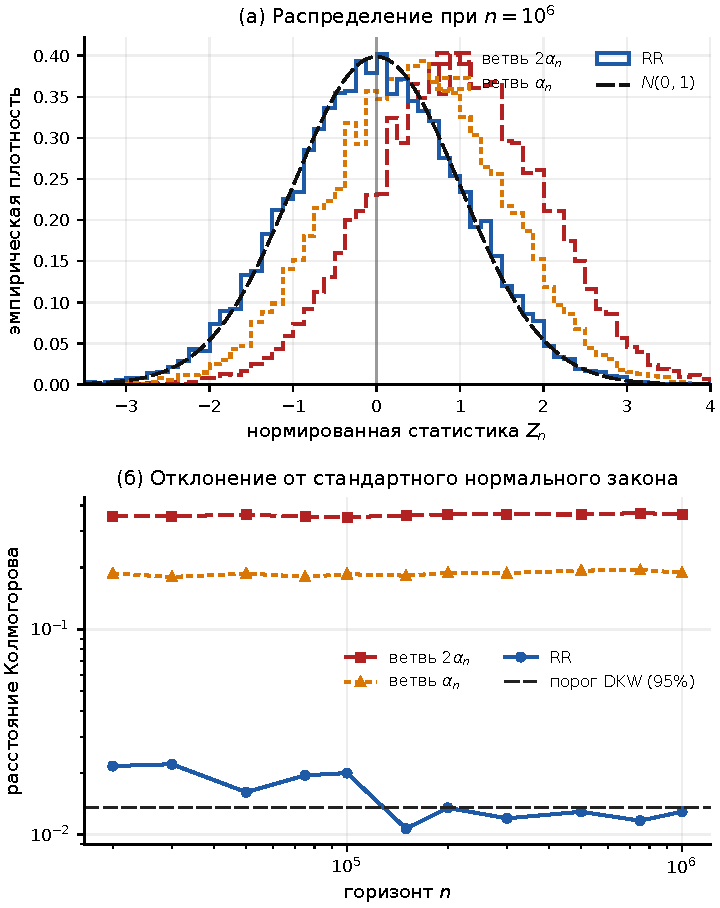
\includegraphics[width=0.90\textwidth]{figures/rr_main_experiment.pdf}
\caption{Главный эксперимент на сбалансированном шаге
$\alpha_n=20/\sqrt n$. Сверху: распределения трёх нормированных статистик
при $n=10^6$. Снизу: расстояние Колмогорова до $N(0,1)$ на 11 горизонтах;
пунктирная линия показывает 95\%-й ориентир выборочной погрешности при
$10\,000$ траекториях.}
\label{fig:main-experiment}
\end{figure}

При $n=10^6$ экстраполяция Ричардсона-Ромберга уменьшает среднее нормированной статистики с $0.482$ и
$0.957$ до $0.006$, тогда как её дисперсия практически не меняется. Поэтому
улучшение нормальной аппроксимации связано именно с коррекцией среднего, а не с
увеличением разброса. Покрытие возрастает до $94.75\%$, а расстояние
Колмогорова уменьшается до $0.0129$.

Та же картина сохраняется на всей сетке: среднее RR-статистики лежит в
интервале $[-0.0207,0.0134]$, тогда как средние отдельных PR-оценок остаются
отделёнными от нуля. Их расстояния Колмогорова также не убывают, в то время
как для RR они находятся в диапазоне $0.0107$--$0.0220$. При
$n\geq150\,000$ наблюдаемое отклонение RR сопоставимо с выборочной
погрешностью для $10\,000$ траекторий. Это не доказывает точную нормальность,
но подтверждает предсказываемый теорией механизм: RR устраняет ведущий сдвиг,
сохраняя масштаб случайных флуктуаций.

\subsection{Устойчивость по шагу и по задачам}

Во втором эксперименте генерируются 100 независимых задач, по 100 траекторий
длины $T=10^6$ для каждой. Цепь стартует из стационарного распределения,
$\thetainit=0$, разогрев равен 1000. Для каждой задачи фиксируется случайное
единичное направление, а пары шагов сравниваются на общих траекториях.
Долгосрочная дисперсия оценивается по 63 неперекрывающимся блочным средним.
В таблице приведены медианы по задачам; $L_2$-ошибка усредняется по
траекториям, а ошибка и ширина указаны в единицах $10^{-3}$.

\begin{table}
\scriptsize
\setlength{\tabcolsep}{2.5pt}
\renewcommand{\arraystretch}{1.18}
\caption{Результаты для 100 случайных задач при $T=10^6$; медианы по
задачам.}
\label{tab:sweep}
\centering
\begin{tabular}{|c|r|r|r|r|r|}
\hline
Пара $(2\alpha,\alpha)$ &
\multicolumn{2}{c|}{Покрытие без RR} &
\multicolumn{3}{c|}{RR} \\
\cline{2-6}
 & $2\alpha$ & $\alpha$ & $L_2$ & Ширина & Покрытие \\
\hline
$(0.04,0.02)$ & 92.0\% & 94.0\% & 2.97 & 5.36 & 94.0\% \\
$(0.10,0.05)$ & 86.0\% & 91.5\% & 2.97 & 5.37 & 94.0\% \\
$(0.20,0.10)$ & 67.5\% & 86.0\% & 2.97 & 5.38 & 94.0\% \\
\hline
\end{tabular}
\end{table}

С ростом шага покрытие отдельных PR-средних снижается с $92.0\%$ до $67.5\%$
для ветви $2\alpha$ и с $94.0\%$ до $86.0\%$ для ветви $\alpha$. Для RR оно
остаётся равным $94.0\%$ при практически неизменных ошибке и ширине. На
наибольшей паре шагов $(0.20,0.10)$ экстраполяция уменьшает медианную
$L_2$-ошибку с $7.53$ и $4.46$ до $2.97$ без расширения интервала.

Замена неперекрывающихся блоков на OBM с $b=\floor{T^{0.6}}$ практически не
меняет результат: для пары $(0.20,0.10)$ медианное и среднее покрытия равны
$95\%$ и $94.6\%$, а ширина составляет $5.42\cdot10^{-3}$. Для
использованного PR-алгоритма с убывающим шагом соответствующие покрытия равны
$92\%$ и $88.9\%$. Тем самым устойчивость RR наблюдается как по шагу, так и
по способу оценки долгосрочной дисперсии.

\subsection{Оракульная и практическая дисперсия}

Последний эксперимент отделяет ошибку центрирования от ошибки оценки
масштаба. Для пары $(0.20,0.10)$ сравниваются интервалы с аналитической
дисперсией $\sigma^2(u)=u^\transpose\Sigma_\infty u$ и стандартной OBM-оценкой
для процесса
$u^\transpose(2\theta_t^{(\alpha)}-\theta_t^{(2\alpha)})$. Используются те же
100 задач и 100 траекторий на задачу, разогрев 1000 и размер блока
$b=\floor{T^{0.6}}$. Таблица содержит медианы по задачам; ширина указана в
единицах $10^{-3}$.

\begin{table}
\footnotesize
\setlength{\tabcolsep}{3pt}
\renewcommand{\arraystretch}{1.15}
\caption{Сравнение оракульной и OBM-нормировки; медианы по задачам.}
\label{tab:oracle}
\centering
\begin{tabular}{|r|l|r|r|r|}
\hline
$T$ & Масштаб & Ширина & Покрытие & Ширина/оракул \\
\hline
$20\,000$ & Оракул & 39.37 & 95.5\% & 1.000 \\
$20\,000$ & OBM    & 37.07 & 94.0\% & 0.942 \\
$10^6$    & Оракул & 5.43  & 95.0\% & 1.000 \\
$10^6$    & OBM    & 5.42  & 95.0\% & 0.998 \\
\hline
\end{tabular}
\end{table}

При $T=20\,000$ OBM несколько недооценивает ширину интервала: отношение к
оракульной ширине равно $0.942$, а покрытие ниже на 1.5 процентного пункта.
При $T=10^6$ отношение ширин достигает $0.998$, и оба метода дают медианное
покрытие $95\%$. Следовательно, на длинных траекториях практическая оценка
масштаба близка к оракульной; основное улучшение по сравнению с отдельными
PR-средними связано с RR-коррекцией центра.

\subsection{Воспроизводимость}

Полные параметры генератора задач и псевдослучайных чисел, соглашение об
индексах при усреднении и точные реализации блочных оценок приведены в
сопровождающем коде.
Для анонимного рецензирования код и агрегированные данные предоставляются
отдельным архивом без истории Git и сведений об авторе.
\AfterPeer{После раскрытия авторства постоянная ссылка на код и данные:
\href{https://github.com/Eviltsundera/Statistical-inference-for-Linear-Stochastic-Approximation-with-Richardson-Romberg-extrapolation/tree/1d7e4d7914c1b0f4c0c5c840418e250e21ae75b5/code/results}
{архив экспериментов}.}

\section{Обсуждение и ограничения}\label{sec:discussion}

Теорема и эксперименты дают согласованную картину. Постоянный шаг быстро
забывает начальное состояние, но создаёт смещение; PR-усреднение уменьшает
вариативность, не исправляя центр. RR использует зависимость двух ветвей
конструктивно: общая траектория сохраняет ведущий шум с коэффициентом
$2-1=1$, а комбинация шагов сокращает первый член разложения смещения.
Пуассоновское разложение затем превращает ведущую взвешенную сумму в
мартингал, а все негауссовские части собираются в один $L_p$-остаток.

Практически это означает следующее. Обе ветви нужно запускать на одной
траектории; выбор шага отвечает прежде всего за центр интервала, а оценка
долгосрочной дисперсии --- за его ширину. Эти две настройки следует
диагностировать раздельно.

У результата есть четыре ограничения.

\begin{itemize}
\item Теорема относится к фиксированным скалярным направлениям. Она не даёт
одновременной гарантии для всех координат и не является многомерной оценкой
Берри--Эссеена.
\item Финальное следствие использует треугольную схему
$\alpha=c/\sqrt n$, разогрев порядка $(\alpha a)^{-1}\log^2n$ и явное
условие $2\alpha\leq\alpha_{\mathrm{adm}}(p,q,\tmix)$. Оно не является
утверждением для фиксированного $\alpha$ без изменения центра.
\item Высокие моменты компонент разложения второго порядка импортируются из
\cite{Levin2026}. Поэтому допустимый шаг зависит от порядка момента $p$, от
$\tmix$ и от условия устойчивости случайных матричных произведений.
\item Близость OBM к оракулу установлена только эмпирически. Состоятельность
OBM для связанной RR-рекурсии, оптимальный размер блока и интервалы с
нормировкой, оценённой по данным, требуют отдельного анализа.
\end{itemize}

Эксперименты используют конечные цепи и умеренную зависимость. Проверка
функции распределения проведена для одной задачи и одного направления, а
популяционный тест --- для 100 задач и 100 траекторий на задачу; поэтому он
проверяет предсказанный механизм, но не заменяет стресс-тестов при медленном
смешивании.

\section*{Заключение}

Для PR-усреднённой после разогрева RR-оценки получена неасимптотическая
нормальная аппроксимация. В допустимом сбалансированном режиме
$\alpha=c/\sqrt n$, $p\asymp\log n$,
$n_0\asymp(\alpha a)^{-1}\log^2n$ и
$2\alpha\leq\alpha_{\mathrm{adm}}(p,q,\tmix)$ основной результат имеет вид
\[
 \dK\!\left(
 \frac{\sqrt n\,u^\top
  (\bar\theta_{n,n_0}^{\RR,\alpha}-\theta^\star)}
      {\sqrt{u^\top\Sigma_\infty u}},
 \mathcal N(0,1)\right)
 \lesssim
 \frac{C_{\mathrm{mix}}(\tmix)\operatorname{polylog}(n)}
      {n^{1/4}}.
\]
Доказательство выделяет ведущий пуассоновский мартингал, сравнивает его
детерминированную ковариационную прокси с $\Sigma_\infty$ и соединяет
опубликованные оценки стационарных компонент с локальной леммой переноса после
разогрева и леммой~\ref{lem:smoothing}.

В численных опытах одиночные ветви сохраняют заметно сдвинутый центр и
недопокрытие, тогда как RR достигает 94--95\%-го покрытия при практически той
же ширине. На длинных траекториях OBM близок к оракульной оценке дисперсии.
Таким образом, шаговая экстраполяция и оценивание долгосрочной дисперсии
являются дополняющими, но различными частями статистического вывода.


\begin{thebibliography}{10}

\Bibitem{RobbinsMonro1951}
\by Robbins~H., Monro~S.
\paper A stochastic approximation method
\jour The Annals of Mathematical Statistics
\yr 1951
\vol 22
\issue 3
\pages 400--407
\doi 10.1214/aoms/1177729586

\Bibitem{ruppert1988efficient}
\by Ruppert~D.
\book Efficient estimations from a slowly convergent Robbins--Monro process
\publ Cornell University Operations Research and Industrial Engineering
\yr 1988

\Bibitem{Dieuleveut2020}
\by Dieuleveut~A., Durmus~A., Bach~F.
\paper Bridging the gap between constant step size stochastic gradient
descent and Markov chains
\jour The Annals of Statistics
\yr 2020
\vol 48
\issue 3
\pages 1348--1382
\doi 10.1214/19-AOS1850

\Bibitem{Polyak1990}
\by Polyak~B.\,T.
\paper A new method of stochastic approximation type
\jour Automation and Remote Control
\yr 1990
\vol 51
\issue 7
\pages 937--946
\mathnet at5521

\Bibitem{PolyakJuditsky1992}
\by Polyak~B.\,T., Juditsky~A.\,B.
\paper Acceleration of stochastic approximation by averaging
\jour SIAM Journal on Control and Optimization
\yr 1992
\vol 30
\issue 4
\pages 838--855
\doi 10.1137/0330046

\Bibitem{Huo2024}
\by Huo~D., Chen~Y., Xie~Q.
\paper Effectiveness of constant stepsize in Markovian LSA and statistical
inference
\jour Proceedings of the AAAI Conference on Artificial Intelligence
\yr 2024
\vol 38
\issue 18
\pages 20447--20455
\doi 10.1609/aaai.v38i18.30028

\Bibitem{Levin2026}
\by Levin~I., Naumov~A., Samsonov~S.
\paper High-order error bounds for Markovian LSA with Richardson--Romberg
extrapolation
\jour Proceedings of the AAAI Conference on Artificial Intelligence
\yr 2026
\vol 40
\issue 43
\pages 36696--36704
\miscnote{\href{https://arxiv.org/abs/2508.05570}{Extended version:
arXiv: 2508.05570}}
\doi 10.1609/aaai.v40i43.40994

\Bibitem{Samsonov2025}
\by Samsonov~S., Sheshukova~M., Moulines~E., Naumov~A.
\paper Statistical inference for linear stochastic approximation with
Markovian noise
\jour Advances in Neural Information Processing Systems
\yr 2025
\vol 38
\miscnote{\href{https://proceedings.neurips.cc/paper_files/paper/2025/hash/ff45bac2fc44064fd8ae85301b40b41e-Abstract-Conference.html}
{Proceedings version}; \href{https://arxiv.org/abs/2505.19102}
{arXiv: 2505.19102}}

\Bibitem{Srikant2024}
\by Srikant~R.
\paper Rates of convergence in the central limit theorem for Markov chains,
with an application to TD learning
\yr 2024
\miscnote{\href{https://arxiv.org/abs/2401.15719}
{arXiv: 2401.15719, version 4 revised in 2026}}

\Bibitem{Wang2026SteadyState}
\by Wang~Z., Wang~Y., Narang~I., Wang~F., Wang~Y., Maguluri~S.,T.
\paper Steady-state behavior of constant-stepsize stochastic approximation:
Gaussian approximation and tail bounds
\yr 2026
\miscnote{\href{https://arxiv.org/abs/2602.13960}{arXiv: 2602.13960}}

\Bibitem{FlegalJones2010}
\by Flegal~J.\,M., Jones~G.\,L.
\paper Batch means and spectral variance estimators in Markov chain Monte
Carlo
\jour The Annals of Statistics
\yr 2010
\vol 38
\issue 2
\pages 1034--1070
\doi 10.1214/09-AOS735

\Bibitem{LiuVatsFlegal2022}
\by Liu~Y., Vats~D., Flegal~J.\,M.
\paper Batch size selection for variance estimators in MCMC
\jour Methodology and Computing in Applied Probability
\yr 2022
\vol 24
\issue 1
\pages 65--93
\doi 10.1007/s11009-020-09841-7

\Bibitem{sutton:book:2018}
\by Sutton, R. S. and Barto, Andrew G.
% edition = {Second},
\jour The MIT Press
% timestamp = {2019-07-13T10:11:53.000+0200},
\paper Reinforcement Learning: An Introduction
\yr 2018

\end{thebibliography}

\makefinish

\English
\maketitle

\end{document}
